
\chapter{Descriptors}\label{descriptors}

\section{introduction}

Over the last decades, image feature detectors and descriptors have become popular tools in the computer vision community,  and they are being applied widely in different applications; image representation, image classification and retrieval, object recognition and matching  3D scene reconstruction, motion tracking   texture classification, robot localization, all rely on the presence of stable and representative features in the image. Thus, detecting and extracting the image features are vital steps for these applications.
Hence the need for a descriptor that can detect and extract features,
and since our HGR system needs a features' detector that can be stable in most cases which will fullfill our need to recognize the gesture performed by the user.


\section{Definitions and principles:}

\subsection{Global and local features}
the following definition was given by krig S in \cite{krig}. 

In the overall feature representation, the image is represented by one multidimensional feature vector which describes the image, in other terms, a single vector that is produced by the global representation method has different values that measure various aspects such as color, shape or texture. Practically we can extract multiple feature vectors from each image that allow us to compare two images. e.g if we want to differentiate sea pictures (blue) and forest pictures (green), a global color descriptor will provide us with different feature vectors of each category. In this context,  global features can be interpreted
as a particular property of image involving all pixels.
This property can be either texture, edges, colors histograms or even a specific descriptor extracted from some filters applied to the image \cite{h}.
On the other side, there is local features that distinctively represent some of the significant regions in the image, these regions remain invariant to viewpoint and intensity changes. 
This property can be color histograms, texture, edges or even a specific descriptor extracted from some filters
applied to the image. Thus, the image is represented
based on its local structures by a set of local feature descriptors which are extracted
from a set of image regions referred to as interest regions (i.e., keypoints), as illustrated in
Fig.\ref{fig:Ft1}

\begin{figure}[H]
\centering
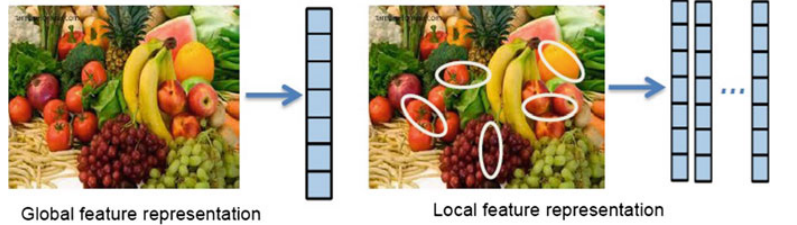
\includegraphics[width=0.9\textwidth]{img/features.PNG}
\caption{ Global and local image features representation }
\label{fig:Ft1}
\end{figure}

In general, the kind of features we choose to use is greatly dependable on the applications on hand. Developers tend to use the most discriminative ones. e.g a person with big nose compared to smaller eyes, and a person with small nose compared to bigger eyes can have similar mug shot in terms of histogram or intensity distribution.\\


Then, local features or the global pattern distilled from local feature clusters seem to be more discriminative. Whereas, for very large datasets in the web scale image indexing application, it is appropriate to consider global features, as they are useful in applications where a rough segmentation of the object of interest is available.
The advantages of global features lay in the fact that they are much faster, are compact and are easy to compute and generally require small amounts of memory.\\ However, the global representation suffers from well known limitations, in particular they are not invariant to significant transformations and are sensitive to clutter and occlusion.\\In some applications, like copy detection, most of the illegal copies are very  similar to the original; they have only suffered from compression, scaling or limited
cropping. In contrast, the advantage of local features is their superior performance \cite{i}. Meanwhile, using local features for large scale image search have much higher performance than global features provide \cite{k}.\\ Besides, as the local structures are more distinctive and stable than other structures in smooth regions, it is probable to be more useful for image matching and object recognition.\\ However, they usually require a significant amount of memory because the image may contain hundreds of local features.\\ Researchers suggest aggregating local image descriptors into a very compact vector representation and optimizing the
dimensionality reduction of these vectors as a solution for this problem. \cite{k}


\subsection{Characteristics of feature detectors}

Tuytelaars and Mikolajczyk \cite{MM} define a local feature as \textit{ “it is an image pattern
which differs from its immediate neighborhood”.} Thus, they consider the purpose of
local invariant features is to provide a representation that allows to efficiently match
local structures between images. That is, we want to obtain a sparse set of local
measurements that capture the essence of the underlying input images and encode
their interesting structures. To meet this goal, the feature detectors and extractors
must have certain properties, keeping in mind that the importance of these properties
depends on the actual application settings and compromises need to be made. The
following properties are important for utilizing a feature detector in computer vision
applications:
\begin{itemize}
\item Robustness, the feature detection algorithm should be able to detect the same feature
locations independent of scaling, rotation, shifting, photometric deformations,
compression artifacts, and noise
\item Repeatability, the feature detection algorithm should be able to detect the same
features of the same scene or object repeatedly under variety of viewing conditions.
\item Accuracy, the feature detection algorithm should accurately localize the image
features (same pixel locations), especially for image matching tasks, where precise
correspondences are needed to estimate the epipolar geometry.
\item Generality, the feature detection algorithm should be able to detect features that
can be used in different applications.
\item Efficiency, the feature detection algorithm should be able to detect features in new
images quickly to support real time applications.
\item Quantity, the feature detection algorithm should be able to detect all or most of the
features in the image. Where, the density of detected features should reflect the
information content of the image for providing a compact image representation.
\end{itemize}

\textbf{in this project We are going to use Local features( descriptors) for its efficiency and scale, rotation  invariant }\\
\section{Spectra descriptors :}
\subsection{SIFT - Scale Invariant Feature Transforms} \label{siftSection}

The Scale Invariant Feature Transform (SIFT) developed by Lowe \cite{lowe}  it is basically the most powerful tool in vision field for detecting and description of interest points in an image, and to identify similar keypoint in different images ( matching ). The idea is these feature provide invariance to scale, rotation, affine distortion, noise,illumination.
the author \cite{lowe} also insisted on using several SIFT descriptors together gives additional invariance to occlusion and clutter. Here are the stages an image passed in order to get a sift descriptor :


\begin{enumerate}
\item Scale-space extrema detection :
The first stage of computation must search over all
scales and image locations, but it can be implemented efficiently by using a difference of-Gaussian
function to identify potential interest points that are invariant to scale and orientation.
\item Keypoint localization :
At each candidate location, a detailed model is fit to determine
location, scale, and contrast. Keypoints are selected based on measures of their
stability.
\item Orientation assignment :
One or more orientations are assigned to each keypoint
location based on local image properties. All future operations are performed relative to the assigned orientation, scale, and location for each feature, providing invariance
to these transformations.
\item Keypoint descriptor  :
The local image gradients are measured at the selected scale
in the region around each keypoint, and transformed into a representation that allows
for local shape distortion and change in illumination.
\end{enumerate}



\subsection{Scale-Space :}

Space scaling  is an important theory in computer vision.
It was developed by Tony Lindeberg in 1994, it allows to analyze an image with a multi-scale approach and to highlight different  structural  sizes in an image.

To create a scale space, SIFT takes the original image, and generates blurred images progressively by applying Gaussian blur.

\begin{align} 
 G(x, y,\sigma )  =\frac{1}{2\pi\sigma^2} e^{\frac{-( x^2 -  y^2)}{2\sigma^2}}
\end{align}


after  blurring images it resizes the original image at half its size and generates again blurred images and so on and so forth.
Images of the same octave are all blurred progressively  with a $\sigma$ (blurring coefficient). An example of the space construction of SIFT scales is presented in Figure \ref{fig:scale}.



\begin{figure}[H]
\centering
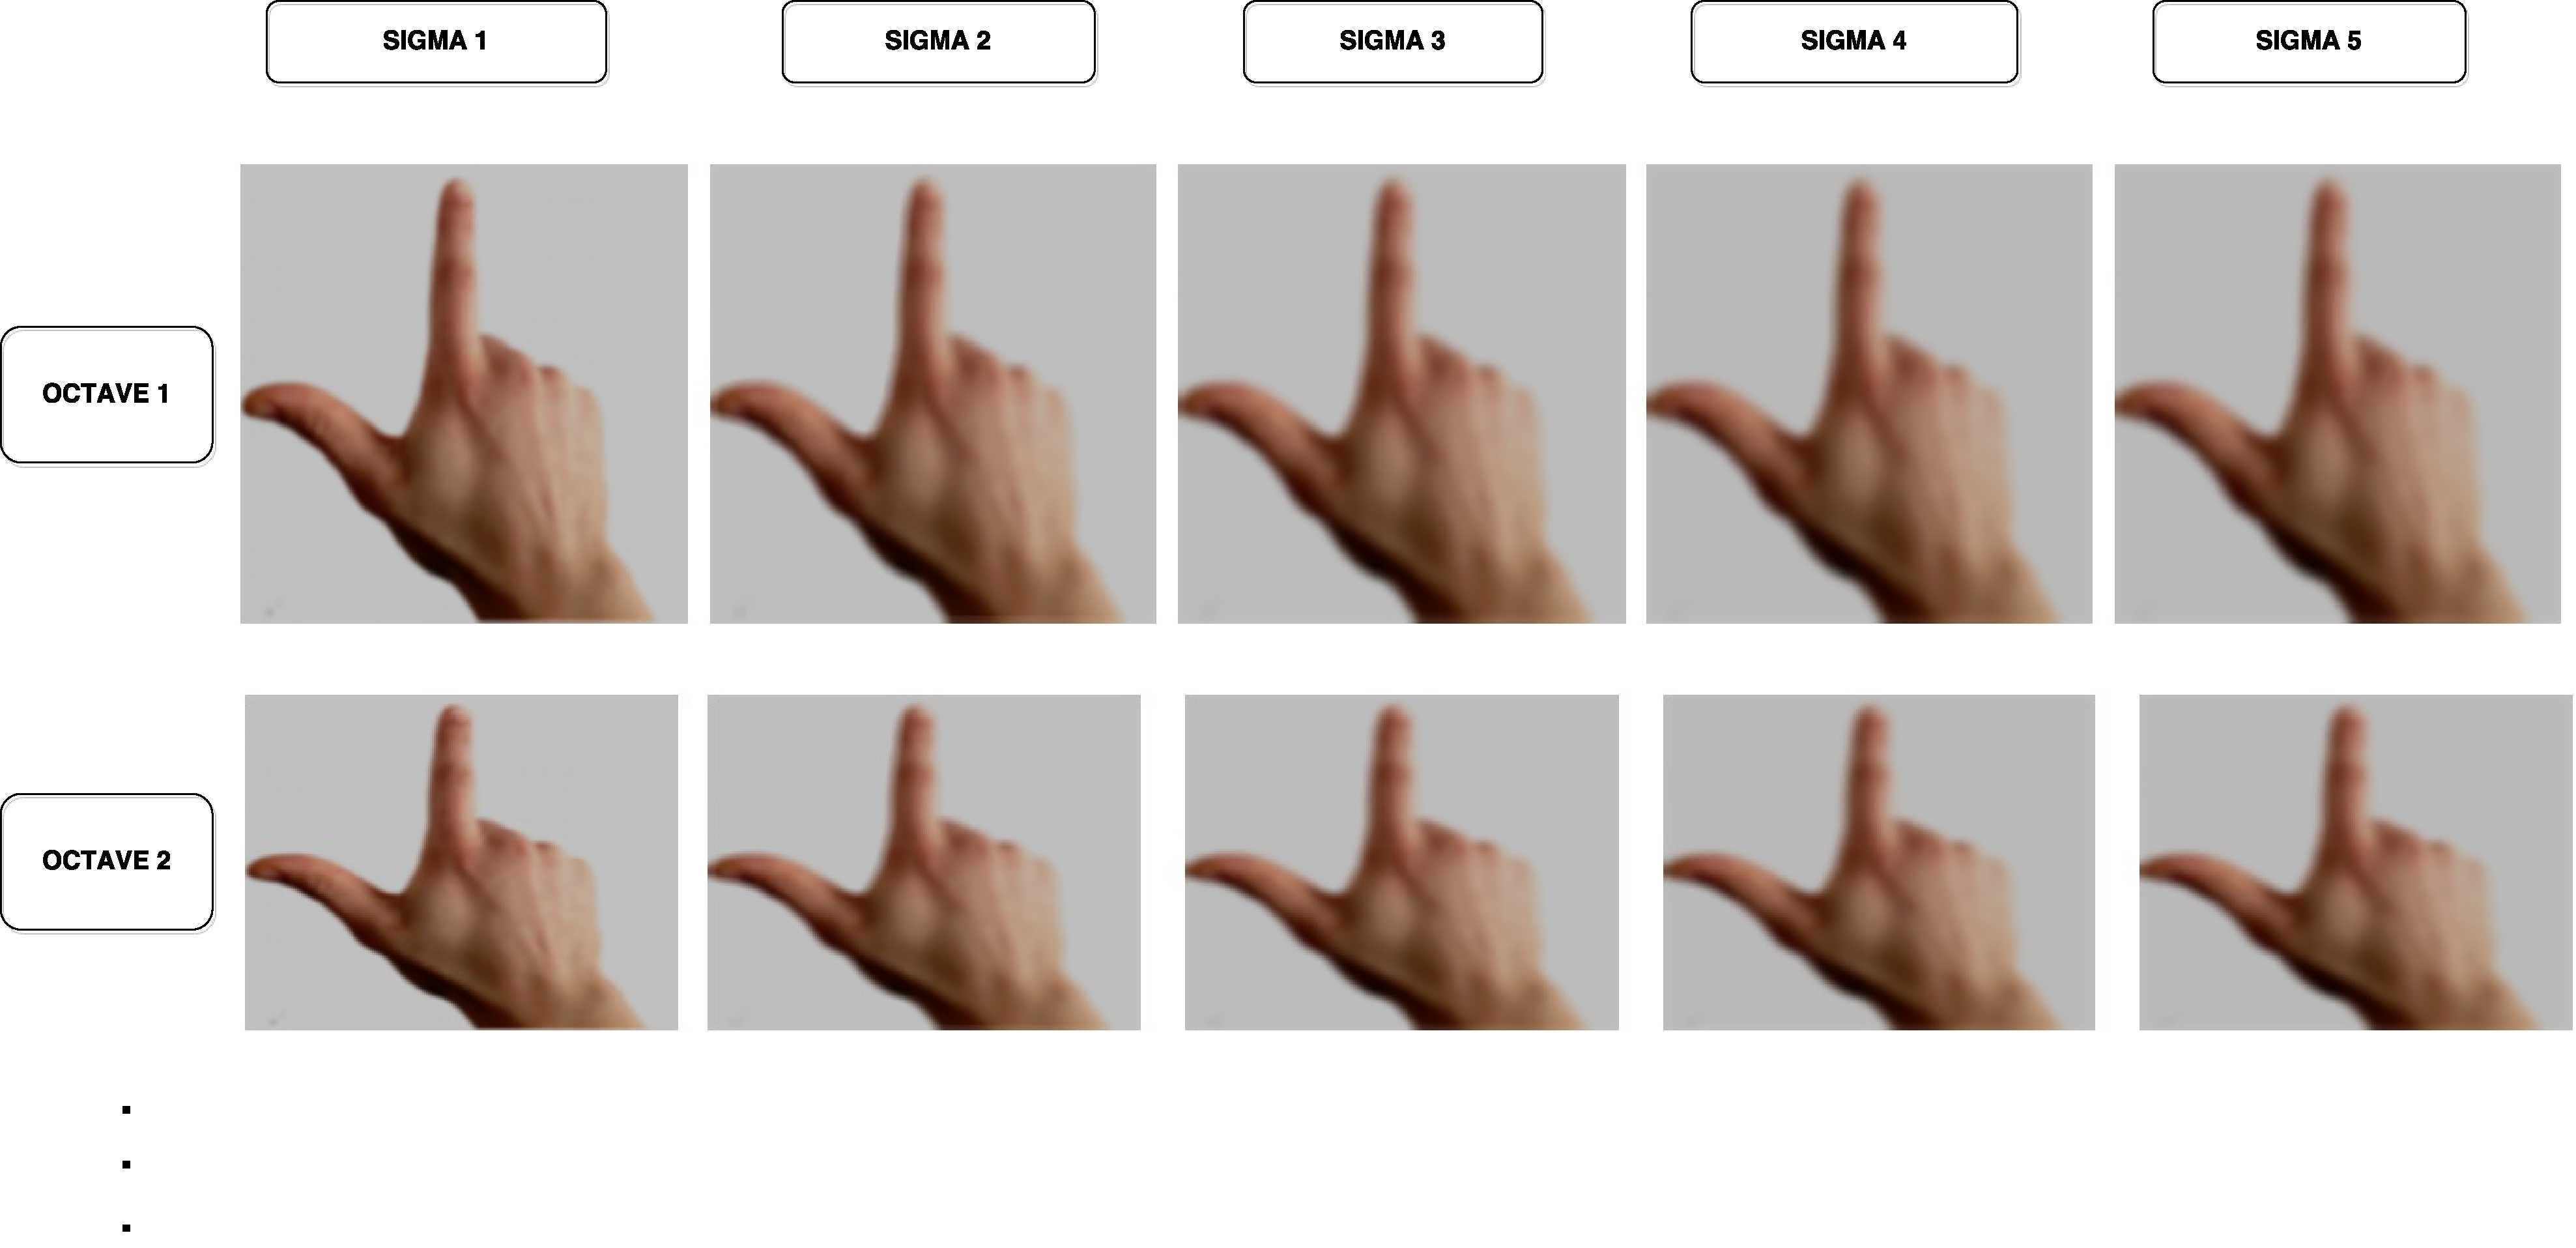
\includegraphics[scale = 0.25]{img/scale_space.pdf}
\caption{ constructing scale space.}
\label{fig:scale}
\end{figure}

\subsection{Detection of Extrema}
In the previous step, we constructed the scale space which consists of image smoothing on several scales and at different sizes. The idea now consists of making a deference of Gaussians (DoG), between two consecutive images of the same octave to obtain DoG images. These [DoGs]  are very useful for the detection of stable Features.


The difference between two consecutive images smoothed by a Gaussian filter constitutes a good approximation of the LoG (Laplacian of Gaussian), a high-pass filter is used to highlight  details that have a fast variation to the brightness  as well as  making the contours  of the objects  visible too, as shown in Figure \ref{fig:sift2}


\begin{figure}[H]
\centering
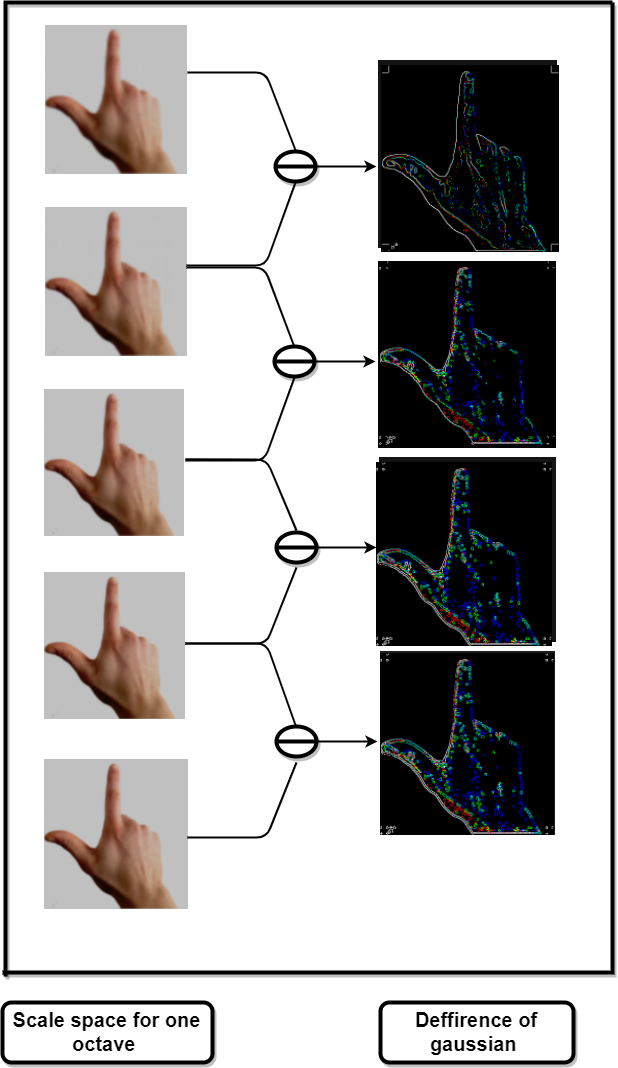
\includegraphics[width=0.5\textwidth]{img/scaleanddog.png}
\caption{ Detection of maxima and minima of the difference-of-Gaussian.}
\label{fig:sift2}
\end{figure}


The keypoints founded by DOG (that are stable) has  locals extremas through the deferent scales. Each pixel of the DoG images is then compared to its 26 neighbors, 8 neighbors in the same scale and 9 neighbors on the two neighboring scales that surround it.

\begin{figure}[H]
\centering
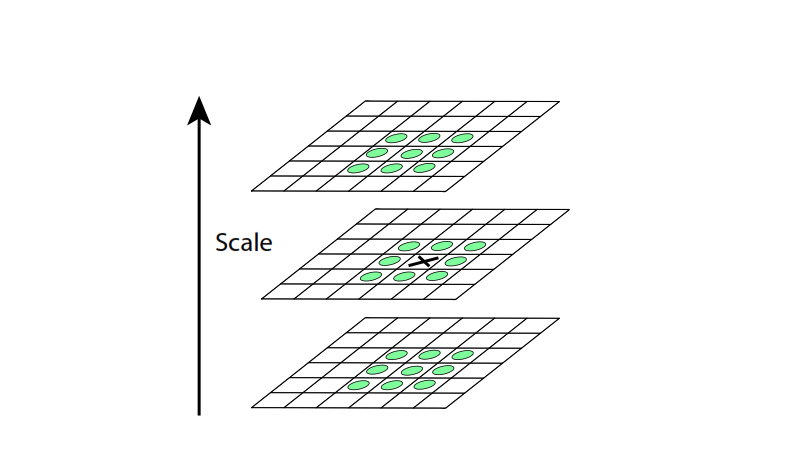
\includegraphics[width=0.5\textwidth]{img/sift2.PNG}
\caption{ Locate maxima/minima in DoG images }
\label{fig:sift4}
\end{figure}
If the pixel  is a local extremas, i.e, if it is greater or lesser  than its neighbors then it is selected as a candidate point for the next steps. This Comparison operation can only be performed for images that have neighboring images above and below.

\subsection{localization  of keypoints and elimination of irrelevant points:}

In general, the extremas detection step produces a large number of keypoint candidates, some of which are unstable;  in addition, their locations in particularly at  the higher scales (i.e. in the upper octaves of the pyramid where resolution is lower) remains approximate. In this step  we will precisely locate the keypoint (the detected extremas), and eliminate the points that have a low contrast and are located on the edges.

The idea is to calculate two gradients at the keypoint, both perpendicular to each other. Based on the image around the keypoint, three possibilities exist. The image around the keypoint can be:
\begin{itemize}

\item A flat region: If this is the case, both gradients will be small.
\item  An edge :  one gradient will be big (perpendicular to the edge) and the other will be small (along the edge)
\item A "corner":  both gradients will be big.
\end{itemize}
Corners are great keypoints. So we want just corners. If both gradients are big enough, we let it pass as a key point. Otherwise, it is rejected.




\subsection{Orientation Assignment }


After these steps we have already eliminated many Keypoints which were likely to be irrelevant to the implementation of the algorithm. Now, it’s a matter of attributing to each detected keypoint 
an orientation by collecting the gradient directions and magnitudes around this keypoint, then figure out the most prominent orientation (note it can be more than just one orientation, either way we assign the most prominent orientations to the detected keypoint). The next figure shows the magnitude and gradient orientations of a keypoint region.

\begin{figure}[H]
\centering
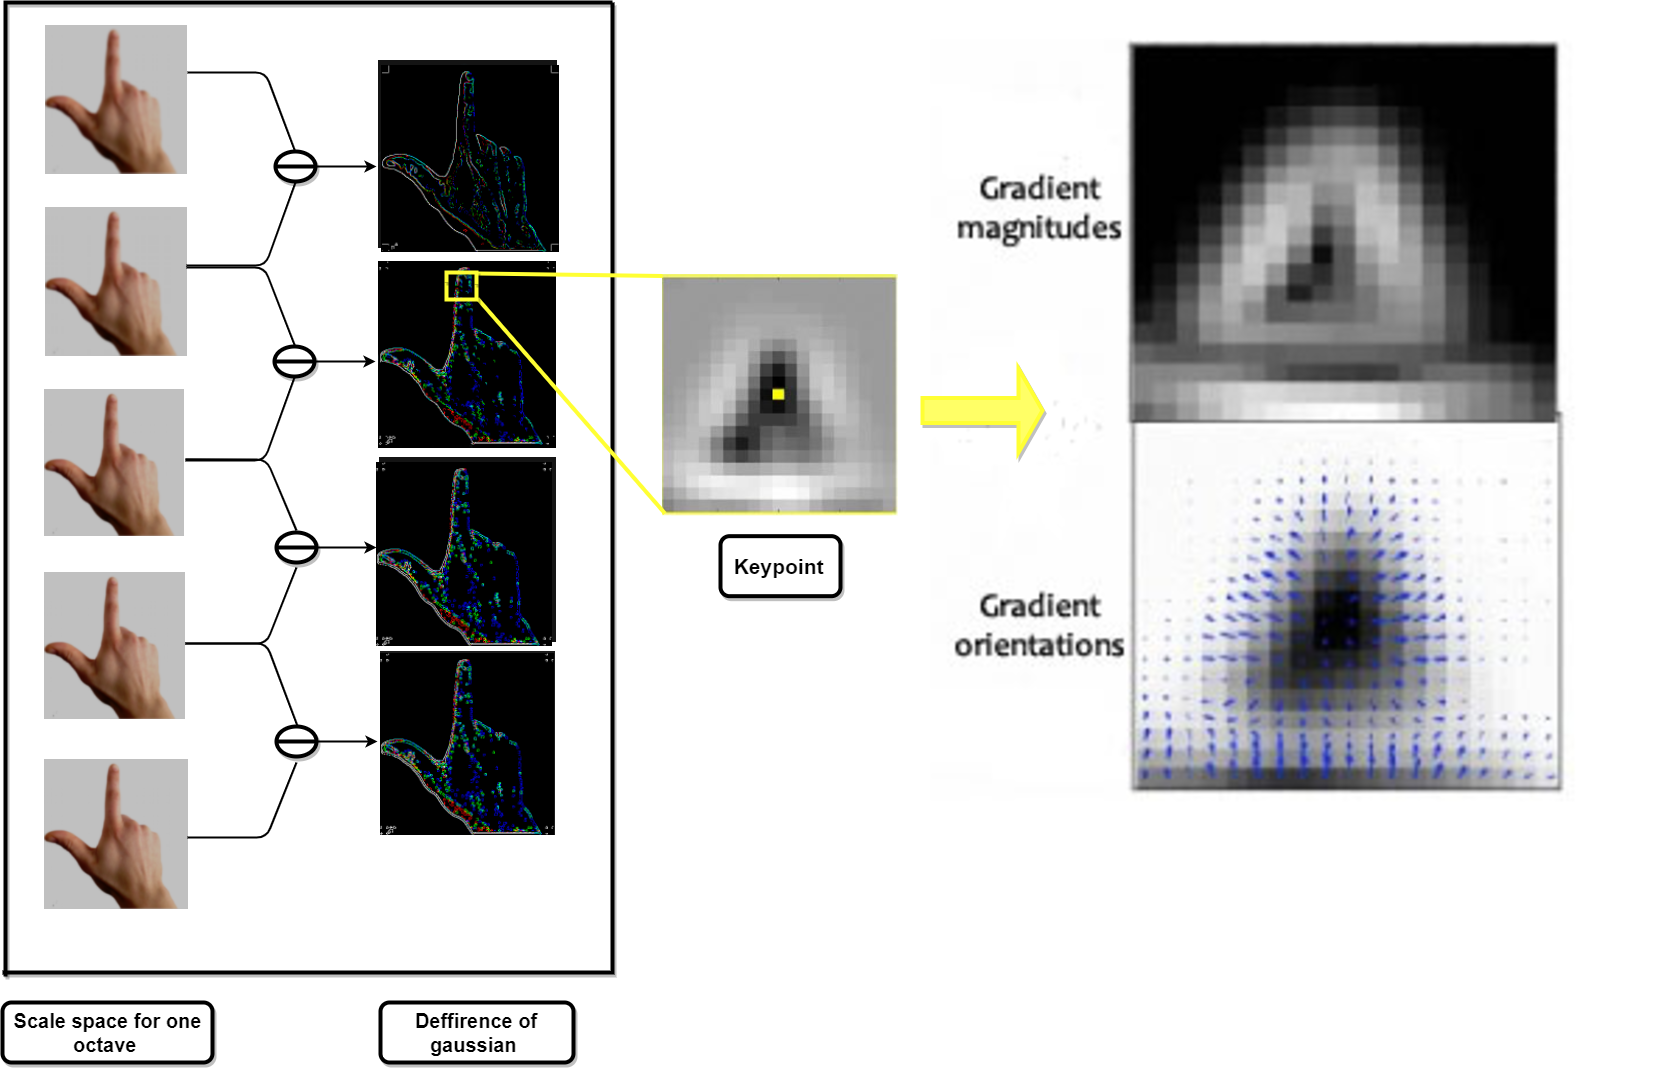
\includegraphics[width=18.5cm, height=13cm]{img/dog_hand.png}
\caption{ calculating Gradient and magnitude in the keypoints neighbor }
\label{fig:orientation}
\end{figure}



The magnitude and orientation is calculated for all pixels around the keypoint. Then, a histogram is created for this.
In this histogram, the 360 degrees of orientation are broken into 36 bins (each 10 degrees). if  the gradient direction at a certain point (in the "orientation collection region") is 18.759 degrees, then it will go into the 10-19 degree bin, and the amount that is added to the bin is proportional to the magnitude of gradient at that point.
then we add a component to the feature  vector of the keypoint that is  defined by (x, y, $\sigma$, $\theta$) where $\theta$ is the orientation of the highest peak in the histogram.

Also, any peaks above 80\% of the highest peak are converted into a new keypoint. This new keypoint has the same location and scale as the original. But it's orientation is equal to the other peak.

\begin{figure}[H]
\centering
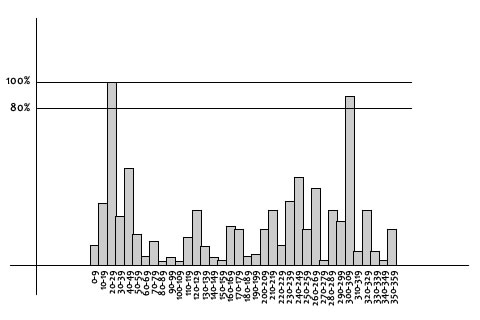
\includegraphics[width=0.8\textwidth]{img/sift_histogram.jpg}
\caption{histogram of magnitude and orientation keypoint region}
\label{fig:histogram}
\end{figure}



In the figure above, you see the histogram peaks at 20-29 degrees. So, the keypoint is assigned orientation 3 (the third bin)

\subsection{keypoint descriptor:}
The last step is to generate a very characteristic [imprint] for each key point. This imprint, a [vector] aims to identify the keypoint, it is unique and tolerant respectfully to the comparison operation. In fact, things are never exactly the same when comparing two different images.
To do this, a 16x16 size window is created around the keypoint. This window is divided into windows of 4x4 size.

\begin{figure}[H]
\centering
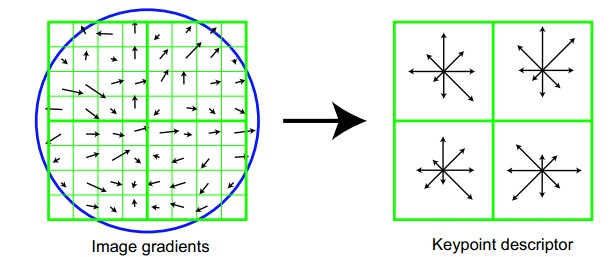
\includegraphics[width=0.8\textwidth]{img/sift4.jpg}
\caption{feature generation}
\label{fig:feature}
\end{figure}


to the first bin. 45-89 add to the next bin. And so on. And the amount added to the bin depends on the magnitude of the gradient. 

Doing this for all 16 pixels within a (4 $\times$ 4) block,we  would gather  16 totally random orientations into 8 predetermined bins.  So you end up with 4$\times$ 4 $\times$8 = 128 numbers. These 128 numbers form the "feature vector". This keypoint is uniquely identified by this feature vector.



\subsection{ SURF ( Speeded Up Robust Features ) }\label{surf}

The detector and descriptor SURF is mainly known for its fast calculations. The comparative study shows the superiority of the SURF detector/descriptor in comparison with SIFT from a point of view of its performances in the execution time and its robustness to luminosity changes [Juan and Gwum, 2009]. In fact, SURF is inspired from SIFT algorithm which is the precursor in the extraction domain of Keypoints. However, the SIFT algorithm has the disadvantage of being slow, which blocks its application in real time.

The approach proposed by SURF uses an approximation of the Hessian matrix in order to detect blobs type structures.  The determinant  of this matrix  can be used to classify the maxima and minima of a function by the second order derivative,  the sign of the  $\det$ (H) can give an idea about local extremum which reprensents the keypoints.

$$ \det (H) =\frac{\partial^2 f \partial^2 f} {\partial x^2 {\partial y^2}}  \bm{-}  (\frac  {\partial^2 f}{\partial x.\partial y})^{2}$$


$
\left\{\begin{matrix}
\ \ \ \ \ \ \det(H) < 0 \Rightarrow  Eijenvalues\ have\ different\ signs\ and\ hence\ the\ point\ is\ not\ a\ local\ extremum.\\
\det(H) > 0 \Rightarrow  both\ Eijenvalues\ have\ same\ signs\ and\ hence\ the\ point\ is\ an\ extremum. 
\end{matrix}\right.
$


Here the hessian matrix is computed at a function of both space X=(x,y) and scale $\sigma$ :



\begin{gather}
 \mathcal{H}(X,\sigma) =
\begin{bmatrix}
                 {L_{xx}(X,\sigma)}  && {L_{xy}(X,\sigma)} \\
                 {L_{xy}(X,\sigma)} && {L_{yy}(X,\sigma)}
\end{bmatrix}
\end{gather}

Where ${L_{xx}(x,\sigma)}$ is the convolution of the Gaussian second order derivative with the image I in point x, and similarly for ${L_{xy}(x,\sigma)}$ and ${L_{yy}(x,\sigma)}$.
First convolution, then second order derivative, the approximation  of Laplacien of Gaussian  (LoG) using box filters for  the respective kernels :

\begin{figure}[H]
\centering
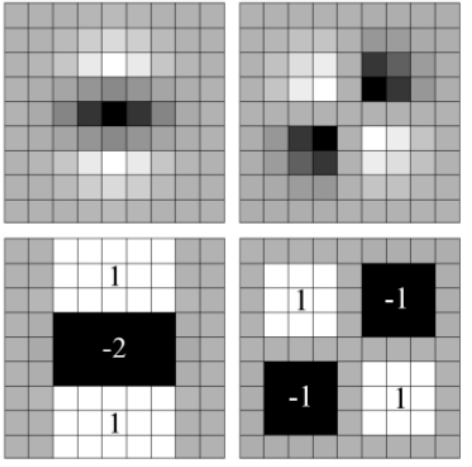
\includegraphics[width=0.55\textwidth]{img/surf4.PNG}
\caption{${L_{yy}(x,\sigma)}$ and${L_{xy}(x,\sigma)}$ Discretized
Gaussians and the approximations $D_{yy}$ and $D_{xy}$}
\label{fig:surf1}
\end{figure}


These approximate second order Gaussian derivatives and can be evaluated at a very low computational cost using integral images, and this is part of the reason why SURF is fast.

Now we can represent the determinant of the Hessian (approximated) as:

\begin{figure}[H]
\centering
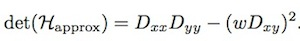
\includegraphics[width= 0.4\textwidth]{img/det.jpeg}

\label{fig:surfdet}
\end{figure}

\subsection{Surf scale space }
Just like SIFT, SURF also created its own scale space.
The scale space is generally implemented as image pyramid (octaves). These images are successively smoothed with a Gaussian and then are sub-sampled in order to attend a high level of the pyramid, (from the largest to the smallest). In  the other hand, SURF proceeds differently in this, In fact, instead of applying successively the same process of Gaussian filtering of each image in  each octave (see SIFT), SURF uses the box-filters of different sizes directly on the integral image. Thus the scale space is built in enlarging the filter rather than iteratively reducing the image size. This enables first to reduce the calculation time, second it allows to avoid aliasing due to sub-sampling of the image.
\begin{figure}[H]
\centering
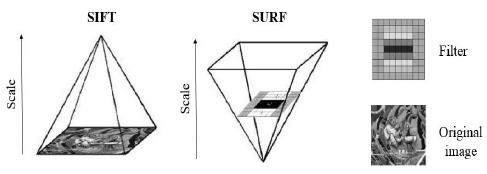
\includegraphics[width=0.6\textwidth]{img/surf2.png}
\caption {The left image represents the classical method with sub-sampling and same filtering. In the image on the right the filters are of various sizes.}
\label{fig:surf2}
\end{figure}


\subsection{Orientation assignment : }

We first calculate the Haar wavelet responses in x and y direction within a circular neighborhood of radius 6s around the interest point, with s the scale at which the interest point was detected. We calculate the sum of vertical and horizontal wavelet responses in a scanning aria, then change the scanning orientation (add $\pi$/3), and recalculate, until we find the orientation with largest sum value, this orientation is the main orientation of feature descriptor.   The size of the Haar filter is 2s. This process makes the descriptor invariant to rotation.

\begin{figure}[H]
\centering
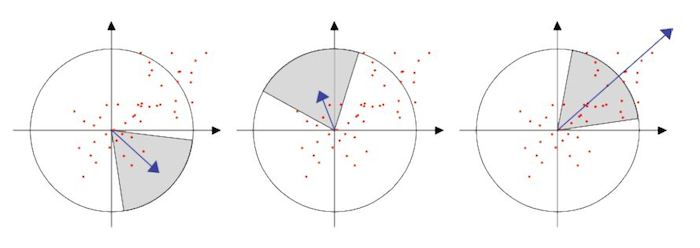
\includegraphics[width=0.6\textwidth]{img/surf3.jpg}
\caption{descriptor computation }
\label{fig:surf3}
\end{figure}

\subsection {Descriptor component : }



The descriptor calculation is done on a squared neighborhood of 20s side, and oriented according to  the largest sum value. The repartition of this neighborhood is identical with the one performed for the SIFT descriptor, i.e 4x4 quadrants.  The dx and dy Haar wavelets are calculated inside each quadrant for a set of 5x5 points. Each quadrant is then characterized by a four components vector.

V=( $\sum dx , \sum \left | dx \right | ,\sum dy , \sum \left | dy \right |$)



\begin{figure}[H]
\centering
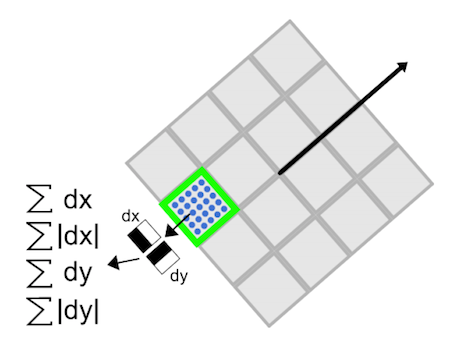
\includegraphics[width=0.5\textwidth]{img/surf5.png}
\caption{computation of dx and dy of Haar  }
\label{fig:surf5}
\end{figure}




The concatenation of these vectors lead to the SURF descriptor of 64 components,
our final descriptor is a 64-D vector. (In Sift, our descriptor is 128-D vector, so this is part of the reason that SURF is faster than Sift.)


\section{Differences and preferences :}
The two main advantages of SURF over SIFT is that SURF uses Laplacian of Gaussian so as to have a distinction
between background and foreground features, and secondly, SURF uses only 64 dimensional vector compared to 128 dimensional vector for SIFT. This helps in fast feature computation and also the quick matching capability.
The two different steps used by SURF to determine the local descriptor vectors are A. Keypoint detection B. Keypoint descriptor, which were  explained above \ref{surf} and \ref{siftSection}.

This makes SURF as our best candidate for gesture recognition  since it offers high number of stable features against scale invariance and rotation invariance, of course lesser than SIFT but it does not worth the computational operations of up scaling pyramid used in sift Nor the \textbf{valuable }time consumed.

Later on we will experimentally demonstrate that SURF achieved  better accuracy than SIFT in hand gesture recognition. However Even if SURF is less expensive than SIFT but still computationally expensive which is bad for our purposes,since what describe a good HGR is its ability to interpret  and interact with the signer performer in real time, That's where Fouriere descriptor appears to give accurate and a very fast feature extractor which will meet our requirement for a robust and real time application.


\section{Fourier shape descriptor } \label{FDT}
The Fourier transformed coefficients from the Fourier
shape descriptors represent the shape of the object in
the frequency domain. The general features of the shape can
be found in the lower frequency descriptors, while the higher
frequency descriptors contain information about the shape
details \cite{20}, before applying Fourier transform on the shape boundary, it is first normalized for matching purposes; this is done by sampling the boundary of each shape to have the same number of data points. The larger the number of sampled points the more details in the representation of the shape,  this results in more accurate matching. While a smaller number of sampled points reduce the accuracy of the matching results but on the other hand it will improve the computational efficiency.
After normalization we  apply Fourier transform to the
shape signature. A shape signature is any 1-D function
representing 2-D areas or boundaries. The shape signature we
used is complex coordinates. A complex coordinates function
is the complex form of the boundary coordinates \cite{20}.
\begin{gather}
    z_{i} = x_{i}+j y_{i} , i\in [1,N]
\end{gather}
For each shape we select N points with equal point
sampling. In order to facilitate the use of Fast Fourier
Transform (FFT), the number of sampled points is chosen to
be power of two. Assuming the number of sampled points is
N the Fourier transform gives N Fourier coefficients Cl. The
coefficients are usually called Fourier descriptors of the shape. 
\begin{gather}
C_{l}= \sum_{i=0}^{N-1} z_{i}e{\frac{-j 2\pi il}{N}} , l = 0,...,N-1
\end{gather}
The magnitude of the Fourier
transform of this set forms a unique shape signature, which can be used for generalized
gesture classification.
In addition, this descriptor is rotationally invariant. Shifts in the silhouette contour
points, which is the cause of rotation, will be appear as phase delays in frequency
domain. However, since only the magnitude of the Fourier coefficients is considered,
the phase (or equivalently, the rotation) is ignored. So, this method is rotationally
invariant while remaining computationally fast\\


\textbf{Generating the Fourier Descriptor: }
\begin{enumerate}
    \item $X_{c} = \frac{1}{N}\sum_{n=0}^{N-1} x(i) , Y_{c} = \frac{1}{N}\sum_{n=0}^{N-1} y(i)  = 1$ , where N is number of hand object pixels 
    \item Take the magnitude of the N point DFT of these points :\\
              \textbf{ abs(FT{r[n]}) = a[m], for m = 0..N-1 }.
    \item Normalize the Fourier coefficients by the DC value (Scale Invariance).
    \item Keep the first 7 normalized coefficients (skip DC, which is always 1).

\end{enumerate}


This is the Fourier descriptor for a single shape.\\

\textbf{Make a dictionary : } For a set of images of the same gesture, compute the average Fourier shape descriptor and add it to the dictionary with the same label.  Repeat for all desired gestures.

\textbf{Classification  : }Compute the Fourier descriptor for each new sample, compare it with each stored gesture in the dictionary using  Euclidean distance measure.  The label of the minimum distance is the desired gesture( nearest neighbor happens to be the most efficient method of classification )


 \section{ Conclusion : }
 In this chapter we went through two types of descriptors:
\textbf{the first} are  Local descriptors SIFT and SURF  descriptors that typically involve more intense computations and algorithms, often requiring floating point calculations, and may consume considerable memory, but generally they give a high  accuracy additionally to their stable performance even against scale variation and Rotation variation too, the following table is summarizing the fifferences of these two descriptors :

\begin{table}[H]
\centering

\begin{tabular}{l|l|l|ll}
\cline{2-3}
\textbf{}                                                                                     & \textbf{SIFT}                                                                                                                                                     & \textbf{SURF}                                                                                                                             &  &  \\ \cline{1-3}
\multicolumn{1}{|l|}{\textbf{\begin{tabular}[c]{@{}l@{}}Keypoint\\ Detection\end{tabular}}}   & \textbf{\begin{tabular}[c]{@{}l@{}}Different scale image\\ convoluted with\\ Gaussian function\end{tabular}}                                                      & \textbf{\begin{tabular}[c]{@{}l@{}}Original Image is\\ convoluted with\\ Different scale box\\ filter\end{tabular}}                       &  &  \\ \cline{1-3}
\multicolumn{1}{|l|}{\textbf{\begin{tabular}[c]{@{}l@{}}Keypoint\\ Description\end{tabular}}} & \textbf{\begin{tabular}[c]{@{}l@{}}Gradient amplitude of\\ a square area is\\ calculated with maximum gradient\\ strength as the main\\ direction\end{tabular}} & \textbf{\begin{tabular}[c]{@{}l@{}}A Haar Wavelet response\\  is used to calculate \\ each sector in a \\ circular area\end{tabular}} &  &  \\ \cline{1-3}
\multicolumn{1}{|l|}{\textbf{Dimensions}}                                                     & 128                                                                                                                                                               & 64                                                                                                                                        &  &  \\ \cline{1-3}
\end{tabular}
\caption{COMPARISON OF SIFT AND SURF}
\label{surfvssift}
\end{table}

\textbf{The second } are basis space descriptors, a basis space is composed of a set of functions, the basis functions, which are
composed together as a set, such as a series like the Fourier series. 

Fourier descriptors represent feature data as sine and cosine terms, which can be
observed in a Fourier power spectrum. The Fourier series, Fourier transform, and fast
Fourier transform are used for a wide range of signal analysis, including 1D, 2D, and 3D
problems. No discussion of image processing or computer vision is complete without
Fourier methods.

With this summary we are done from Feature detection / extraction and we will move on to the next phase of building  our HGR System, which is  feature classification using Machine learning algorithms that's going to be the goal of next chapter.